\documentclass[12pt]{article}
\usepackage[12pt]{moresize}

\usepackage{amsmath}
\usepackage{amssymb}

\usepackage{graphicx}
\usepackage{subcaption}

\usepackage{algorithm}
\usepackage{algpseudocode}
\usepackage{alltt}

\usepackage{multicol}

\usepackage[margin=1in]{geometry}

%\usepackage{hyperref}
%\usepackage[latin1]{inputenc}
%\usepackage{listings}
%\usepackage{scrextend}
%\usepackage{changepage} %Adjustwidth



\title{Stat 330\\Homework 2}
\author{Sean Gordon}
%\date{09/09/2019}

\begin{document}
\maketitle


\hrulefill \\


\noindent 1)\\
\indent (a) $|\Omega| \ge |A|,\ \ |\Omega| \ge 0,\ \ $ therefore $ |A| \div |\Omega| \ge 0$. \\
\indent This satisfies the first axiom.\\

(b) By definition, the sum of the probabilities of all outcomes ( P(A) ) is one, \\
\indent satisfying the second axiom.\\

(c)\\

\hrulefill \\


\noindent 2)\\
\indent (a) 12 * 11 * 10 = 1320 possible permutations\\

\indent (b) 1320 possible permutations, 3 * 2 * 1 = 6 orders per group\\
\indent \indent 1320 / 6 = 220 possible combinations.\\

\indent (c) 3 * 2 * 1 = 6 possible permutations\\


\hrulefill \\
\pagebreak


\noindent 3)\\
\indent (a) 26 + 26 + 3 = 55 letters, 10 numbers.\\
\indent \indent 55 + 10 = 65 possible options per character.\\
\indent \indent 65{\large$^8$} = 3.186448129*10{\large$^{14}$} possible passwords.\\\\
\indent \indent Remove all with no letters (10{\large$^8$}) and those with no numbers (55{\large$^8$}),\\
\indent \indent resulting in 2.34910775*10{\large$^{14}$} possible permutations. \\
\indent \indent This rounds to 235 trillion permutations.\\


\hrulefill \\


\noindent 4)\\
\indent (a) 8 * 7 * 6 * 5 * 4 * 3 * 2 * 1 = 8! = 40320 possible ways.\\

\indent (b) Removing two letter choices effectively makes this a 6 letter word, \\
\indent thus there are 6! = 720 possible ways.\\

\indent (c) 720 $\div$ 40320 = 1.79\% \\


\hrulefill \\
\pagebreak


\noindent 5) For a probability $\ge$ .5, there must be at least 23 people in a room 
\begin{figure}[h!]
  \centering
  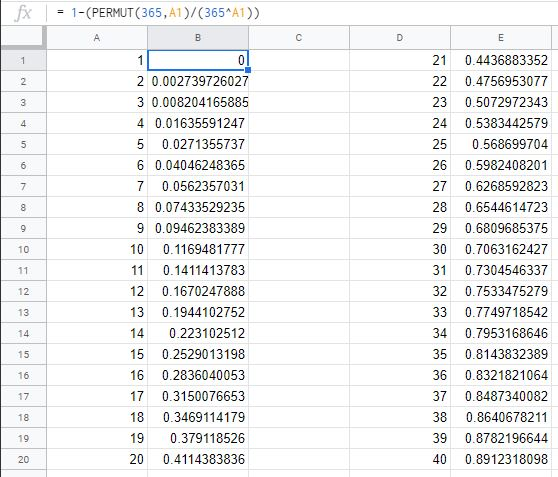
\includegraphics[scale=.8]{Q5.JPG}
\end{figure}




\hrulefill \\


\noindent 6)\\
\indent (a) {\Large $({7 \choose 4}{4 \choose 0}{1 \choose 0})\div{12 \choose 4}$} = 35 $\div$ 495 = 7.1\% chance\\

\indent (b) {\Large $({7 \choose 1}{4 \choose 2}{1 \choose 1})\div{12 \choose 4}$} = 42 $\div$ 495 = 8.5\% chance\\

\indent (c) P(At least 1 Comet) = 1 - P(No Comets):\\
\indent \indent  {\Large $({5 \choose 4})\div{12 \choose 4}$} = 1 - (5 $\div$ 495) = 98.99\% chance\\


\end{document}
















